\documentclass[a4paper, 12pt]{article}
\usepackage[UTF8]{ctex}
\title{实验报告}
\author{23020007067 李子昊}
\date{\today}
\usepackage{color}    
\usepackage{float}
\usepackage{graphicx}
\usepackage[left=2cm,right=2cm,top=2cm,bottom=2cm,head=1cm,headsep=0.5cm,foot=1cm]{geometry}
\usepackage{hyperref}
\usepackage{indentfirst}
\hypersetup{hidelinks,
	colorlinks=true,
	allcolors=black,
	pdfstartview=Fit,
	breaklinks=true}
    
\begin{document}
\maketitle

\pagenumbering{roman}
\large \tableofcontents
\newpage
\pagenumbering{arabic}
 
 \section{课后练习}
 \subsection{练习内容}
 \noindent 1.如果您之前从来没有用过 Git,推荐您阅读 Pro Git 的前几章,或者完成像 Learn Git Branching 这样的教程。重点关注 Git 命令和数据模型相关内容;
 \\ 
2.克隆本课程网站的仓库
 
\indent 2.1将版本历史可视化并进行探索


\indent 2.2是谁最后修改了 README.md 文件?(提示:使用 git log 命令并添加合适的参数)\\
\indent 2.3最后一次修改 \_config.yml 文件中 collections: 行时的提交信息是什么?(提示:使用 git blame 和 git show)
\\


 \subsection{练习结果}
1.习题一:克隆版本控制网址(Git)的仓库
 \begin{figure}[H]
  \centering
  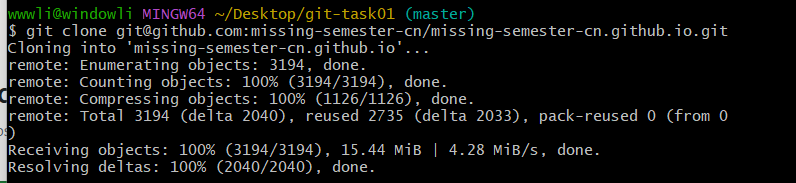
\includegraphics[width=1\textwidth]{屏幕截图 2024-08-28 164453.png}
  \caption{1}
    \end{figure}

 2习题二:\\
   2.1\quad 将'git log --pretty=oneline --all --graph --abbrev-commit'取别名并且查看历史版本。
   \begin{figure}[H]
  \centering
  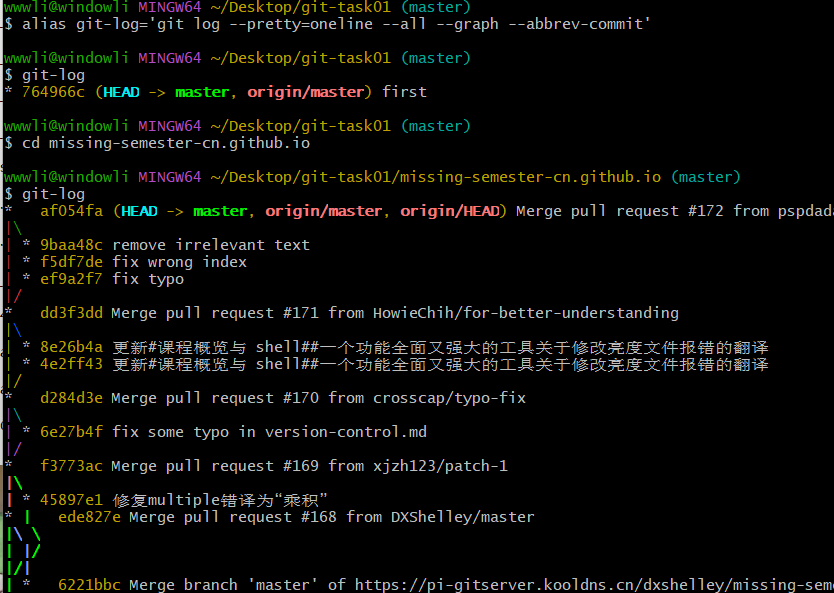
\includegraphics[width=1\textwidth]{屏幕截图 2024-08-28 164831.png}
  \caption{2.1}
    \end{figure}
2.2 \quad 查看README.md文件的最近一次修改
\begin{figure}[H]
  \centering
  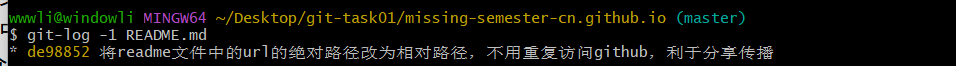
\includegraphics[width=1\textwidth]{屏幕截图 2024-08-28 165007.png}
  \caption{2.2}
    \end{figure}
    \\

    2.3\quad 查看某个文件的最近一次修改了什么信息
\begin{figure}[H]
  \centering
  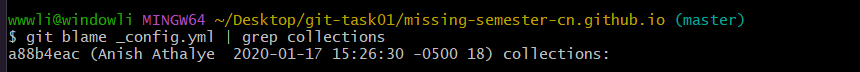
\includegraphics[width=1\textwidth]{屏幕截图 2024-08-28 165107.png}
  \caption{2.3}
    \end{figure}

\section{git实例}
\subsection{git实例展示}
%\listoffigures

 
  \\
   
%\colorbox{red}{one two three}
  
\begin{table}[H]
\centering
\caption{ {\color{red}git实例展示}}
\begin{tabular}{cll}
1&git clone &克隆仓库    \\
2&git remote add origin & 将本地与远端连接    \\
3&alias git-log='git log --pretty=oneline ' &  取别名   \\
4& git-log -1 README.md &  查看某个文件的最近一次修改   \\
5&git blame _config.yml | grep collections &   查看某个文件的最近一次修改了什么信息  \\
6&git remote -v &   查看远程版本库信息  \\
7&git pull origin master &  下载代码并且快速合并   \\
8&git branch dev1 &  创建分支   \\
9&git branch -d dev1 &    删除分支 \\
10&git tag li &   创建标签  \\
 11& git tag -d li& 删除标签   \\
 12&git merge dev1 & 合并分支   \\
 13&git mv file1.txt file2.txt & 文件改名  \\
 14&git rm --cached file2.txt & 停止跟踪文件但不删除  \\
 15& git commit --amend& 修改最后一次提交   \\
 16&git push origin master & 上传代码并且快速合并  \\
 17&git pull origin master --allow-unrelated-histories & 将远程分支合到当前分支   \\
 18&git fetch origin master & A  从远端仓库获取 \\
 19&git push -f --set-upstream origin master:master &  强制上传至远程  \\
 20&git branch & 查看分支 
\end{tabular}
\end{table}


  %1.克隆版本控制网址(Git)的仓库。
  \begin{figure}[H]
  \centering
  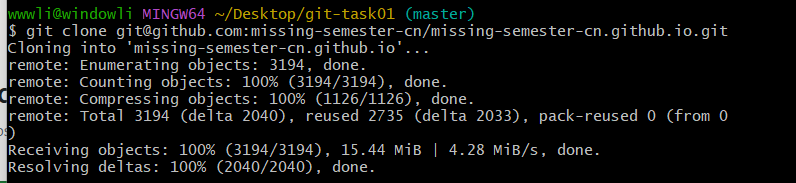
\includegraphics[width=1\textwidth]{屏幕截图 2024-08-28 164453.png}
  \caption{克隆版本控制网址(Git)的仓库}
    \end{figure}

 \\



%2.将本地仓库与远端仓库连接并将本地仓库内容传到远端。

     % \href{https://github.com/newbeginnerlzh/git-task01.git}{https://github.com/newbeginnerlzh/git-task01.git}
\begin{figure}[H]
  \centering
  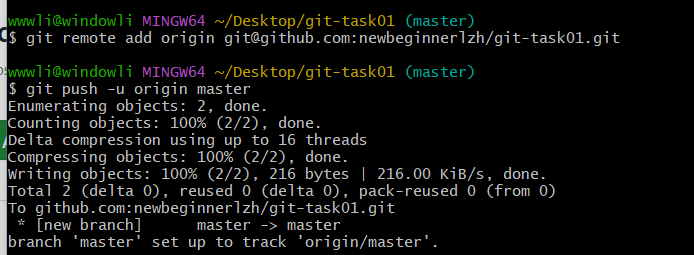
\includegraphics[width=1\textwidth]{屏幕截图 2024-08-28 164514.png}
  \caption{将本地仓库与远端仓库连接并将本地仓库内容传到远端。\href{https://github.com/newbeginnerlzh/git-task01.git}{\color{red}https://github.com/newbeginnerlzh/git-task01.git}}
    \end{figure}
\\



\\
%3.将'git log --pretty=oneline --all --graph --abbrev-commit'取别名并且查看历史版本。
\begin{figure}[H]
  \centering
  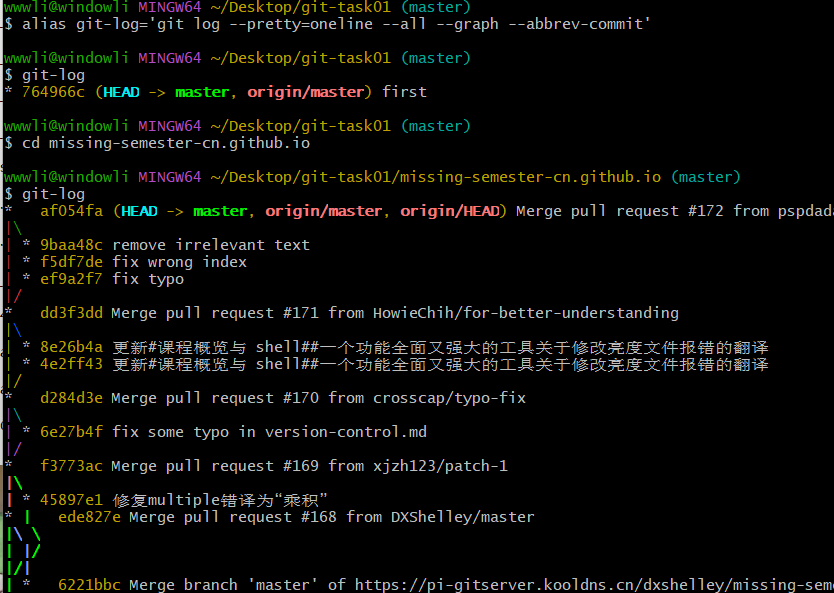
\includegraphics[width=1\textwidth]{屏幕截图 2024-08-28 164831.png}
  \caption{将'git log --pretty=oneline --all --graph --abbrev-commit'取别名并且查看历史版本。}
    \end{figure}
\\
 \\   
%4.查看某个文件的最近一次修改。
\begin{figure}[H]
  \centering
  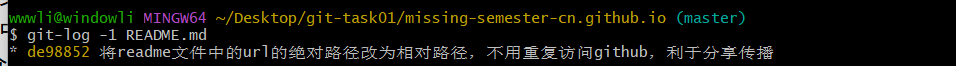
\includegraphics[width=1\textwidth]{屏幕截图 2024-08-28 165007.png}
  \caption{查看某个文件的最近一次修改}
    \end{figure}
\\
\\
\\
%5.查看某个文件的最近一次修改了什么信息。
\begin{figure}[H]
  \centering
  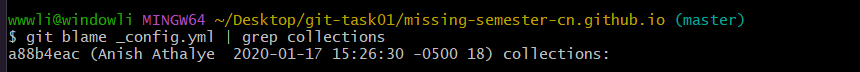
\includegraphics[width=1\textwidth]{屏幕截图 2024-08-28 165107.png}
  \caption{查看某个文件的最近一次修改了什么信息}
    \end{figure}
\\
  \\
  \\

\begin{figure}[H]
  \centering
  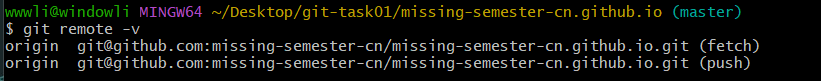
\includegraphics[width=1\textwidth]{屏幕截图 2024-08-28 192417.png}
  \caption{查看远程版本库信息}
    \end{figure}

    
    \begin{figure}[H]
  \centering
  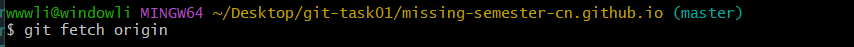
\includegraphics[width=1\textwidth]{屏幕截图 2024-08-28 192431.png}
  \caption{从远程库中获取代码}
    \end{figure}

    
    \begin{figure}[H]
  \centering
  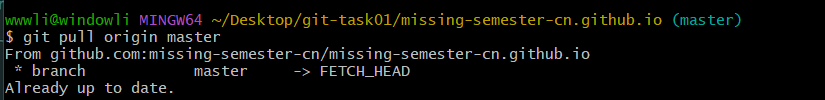
\includegraphics[width=1\textwidth]{屏幕截图 2024-08-28 192444.png}
  \caption{下载代码并且快速合并}
    \end{figure}

     \begin{figure}[H]
  \centering
 
  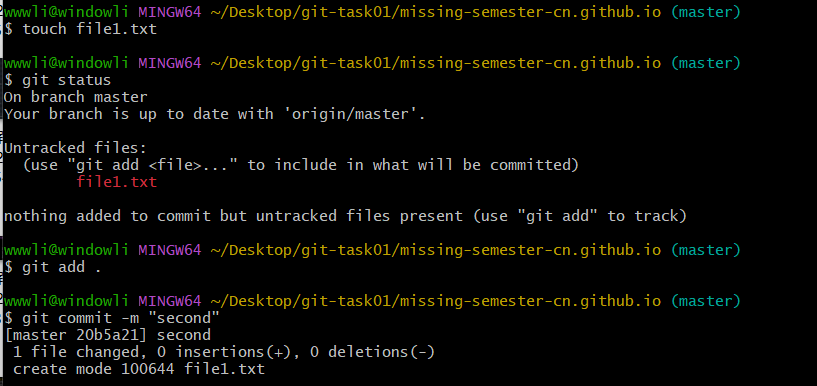
\includegraphics[width=1\textwidth]{屏幕截图 2024-08-28 194414.png}
     \caption{创建文件并将其保存到本地仓库}
    \end{figure}
\\
\\


 \begin{figure}[H]
  \centering
  
\includegraphics[width=1\textwidth]{屏幕截图 2024-08-28 194436.png}
  \caption{用vi编译文本文件}
    \end{figure}
  \\
  \\  
  
  \begin{figure}[H]
  \centering
  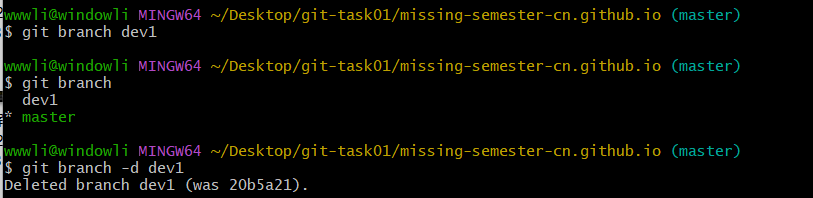
\includegraphics[width=1\textwidth]{屏幕截图 2024-08-28 194454.png}
  \caption{创建分支、显示分支、删除分支}
    \end{figure}
 \\
  \\  
  \begin{figure}[H]
  \centering
  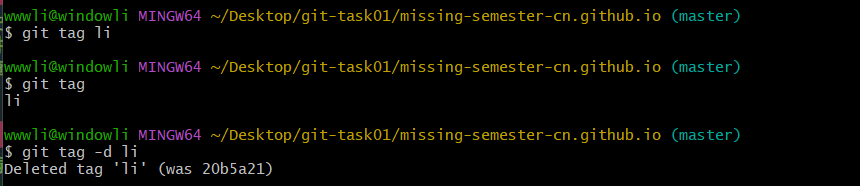
\includegraphics[width=1\textwidth]{屏幕截图 2024-08-28 195638.png}
  \caption{创建标签、显示标签、删除标签}
    \end{figure}
    
    \begin{figure}[H]
  \centering
  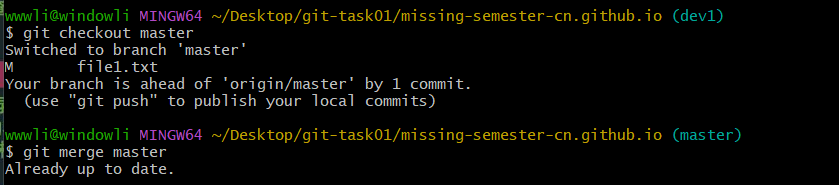
\includegraphics[width=1\textwidth]{屏幕截图 2024-08-28 201335.png}
  \caption{切换分支,合并分支}
    \end{figure}

 \begin{figure}[H]
  \centering
  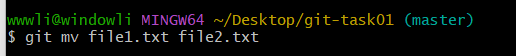
\includegraphics[width=1\textwidth]{屏幕截图 2024-08-29 100431.png}
  \caption{文件改名}
    \end{figure}
    
 \begin{figure}[H]
  \centering
  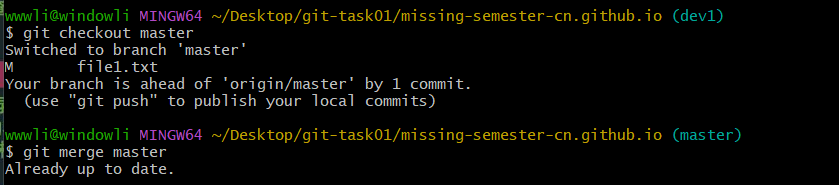
\includegraphics[width=1\textwidth]{屏幕截图 2024-08-28 201335.png}
  \caption{停止跟踪文件但不删除}
    \end{figure}


    \begin{figure}[H]
  \centering
  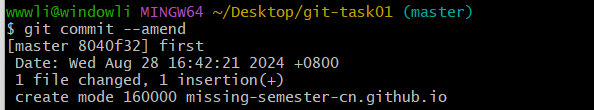
\includegraphics[width=1\textwidth]{屏幕截图 2024-08-29 100548.png}
  \caption{修改最后一次提交}
    \end{figure}

      \begin{figure}[H]
  \centering
  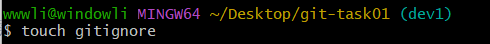
\includegraphics[width=1\textwidth]{屏幕截图 2024-08-29 103132.png}
  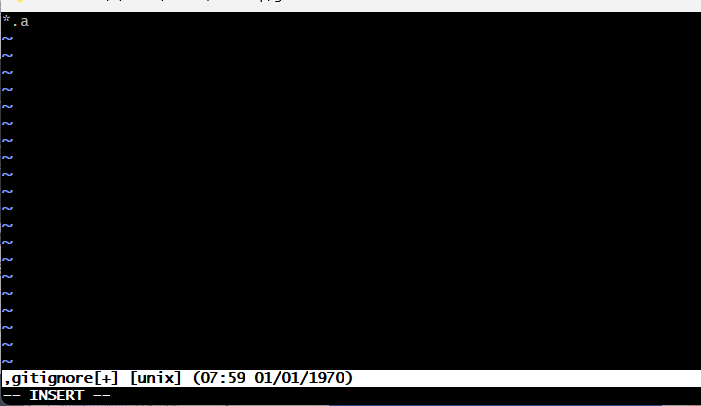
\includegraphics[width=1\textwidth]{屏幕截图 2024-08-29 102427.png}
  \caption{添加文件到忽略列表}
    \end{figure}

    

    \begin{figure}[H]
  \centering
  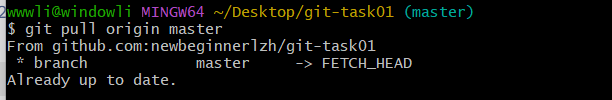
\includegraphics[width=1\textwidth]{屏幕截图 2024-08-29 114216.png}
  \caption{下载代码并且快速合并}
    \end{figure}

    
    \begin{figure}[H]
  \centering
  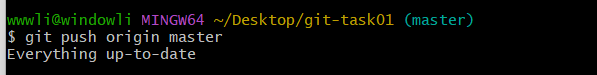
\includegraphics[width=1\textwidth]{屏幕截图 2024-08-29 114230.png}
  \caption{上传代码并且快速合并}
    \end{figure}

 \begin{figure}[H]
%  \centering
  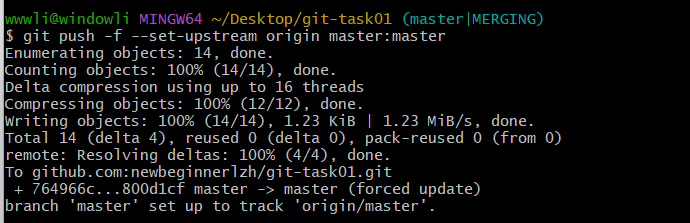
\includegraphics[width=1\textwidth]{屏幕截图 2024-08-29 112519.png}
  \caption{强制将本地仓库上传至远程}
    \end{figure}



\subsection{git个人心得}
    {\color{blue}通过学习了git,我掌握了版本控制的核心概念,这为代码管理提供了强大的工具。}Git允许我们轻松地跟踪项目的所有变化,回溯到任何一个历史版本,并在多人协作时避免冲突。理解分支和合并的工作原理,可以帮助我们更好地组织和协调项目开发,避免开发过程中可能遇到的混乱。
    \\
    \indent  {\color{red}在我的实际使用中,认识到了频繁提交(commit)的重要性,每次提交都是一个小而完整的变更。}这不仅有助于更清晰地理解项目的历史,还能够在出现问题时快速定位问题的根源。通过编写有意义的提交信息,可以更轻松地理解每次变更的意图和目的。
\\
    \indent  {\color{green}最后,我认为Git的协作功能如pull request和代码审查使得团队开发更加高效。}通过定期同步(pull)和推送(push),团队成员能够保持代码库的一致性。同时,利用Git的分支策略,可以为新功能、修复Bug或试验性开发创建独立的环境,确保主代码库的稳定性。

\section{latex实例}
\begin{table}[H]
\centering
\caption{ {\color{red}latex实例展示}}
\begin{tabular}{cl}
1&创建目录    \\
2 & 创建章节   \\
3&引用图片   \\
4& 使用usepackage   \\
5&添加标题、作者、日期  \\
6&创建表格  \\
7&改变字体颜色   \\
8&调整字体大小   
\end{tabular}
\end{table}

\subsection{latex实例展示}


\begin{figure}[H]
  \centering
  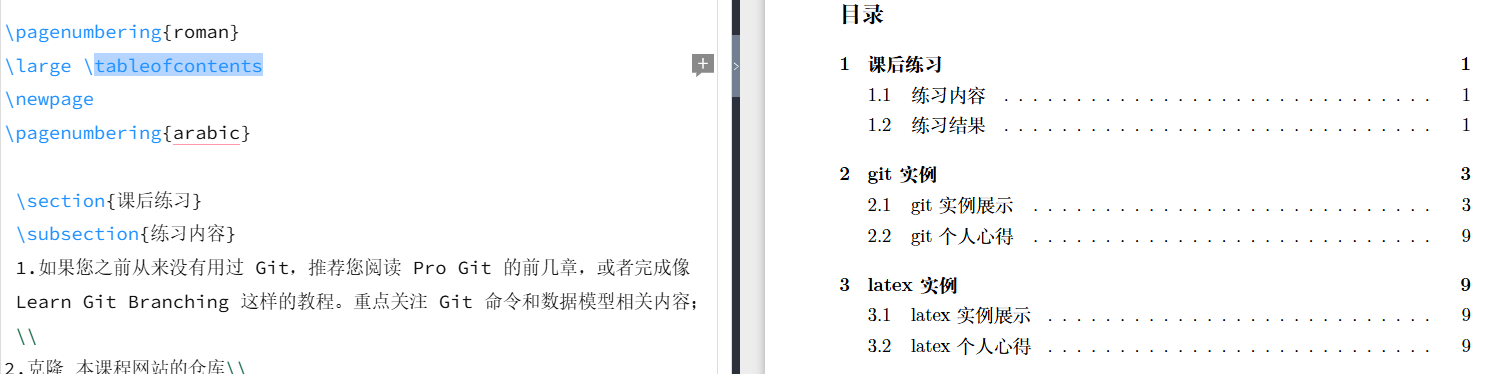
\includegraphics[width=1\textwidth]{屏幕截图 2024-08-29 193720.png}
  \caption{创建目录}
    \end{figure}
\\    
    \begin{figure}[H]
  \centering
  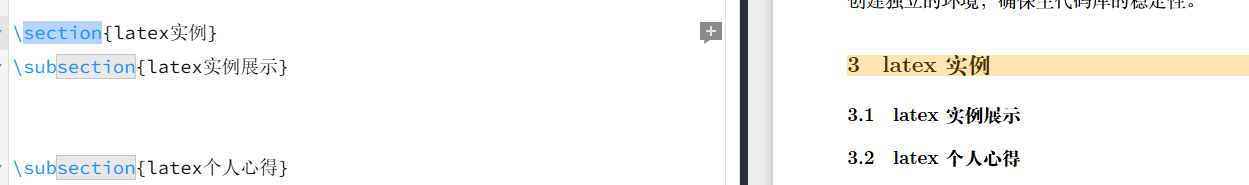
\includegraphics[width=1\textwidth]{屏幕截图 2024-08-29 193915.png}
  \caption{创建章节}
    \end{figure}
\\
\begin{figure}[H]
  \centering
  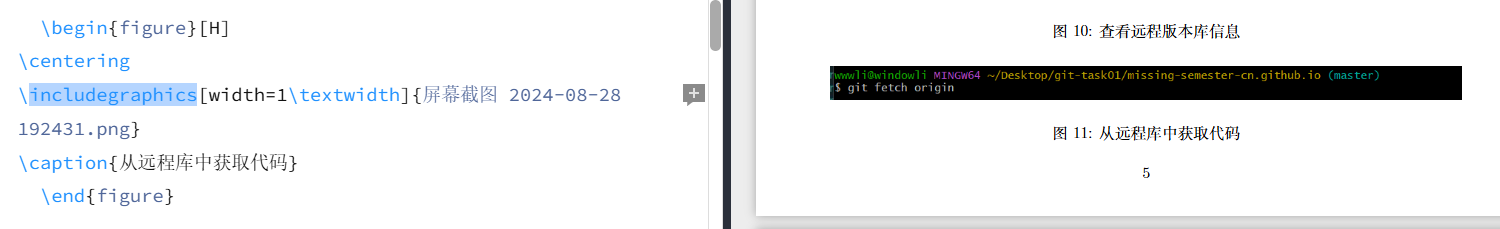
\includegraphics[width=1\textwidth]{屏幕截图 2024-08-29 193853.png}
  \caption{引用图片}
    \end{figure}
 \\   
    \begin{figure}[H]
  \centering
  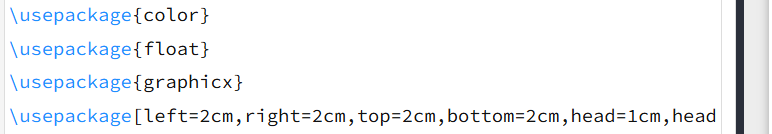
\includegraphics[width=1\textwidth]{屏幕截图 2024-08-29 194021.png}
  \caption{使用usepackage}
    \end{figure}
\\
\begin{figure}[H]
  \centering
  
\includegraphics[width=1\textwidth]{屏幕截图 2024-08-29 194006.png}
  \caption{添加标题作者日期}
    \end{figure}
\\
    \begin{figure}[H]
  \centering
  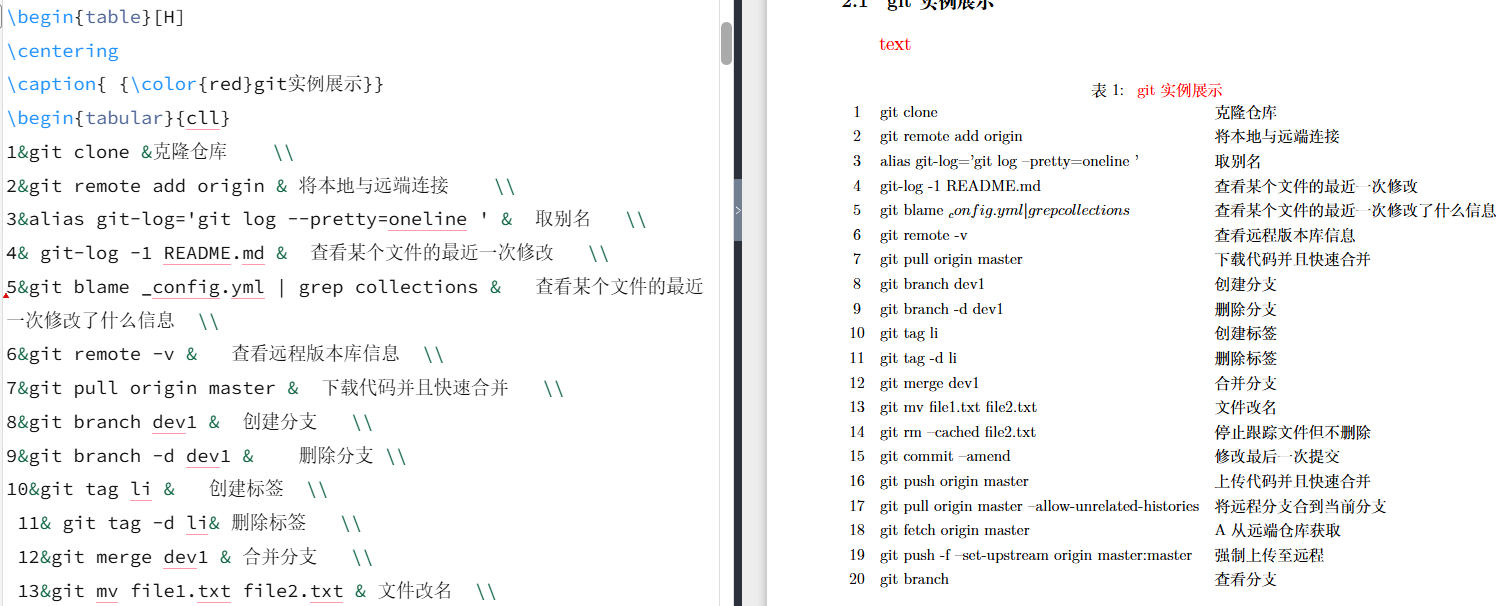
\includegraphics[width=1\textwidth]{屏幕截图 2024-08-29 201017.png}
  \caption{创建表格}
    \end{figure}
\\
    \begin{figure}[H]
  \centering
  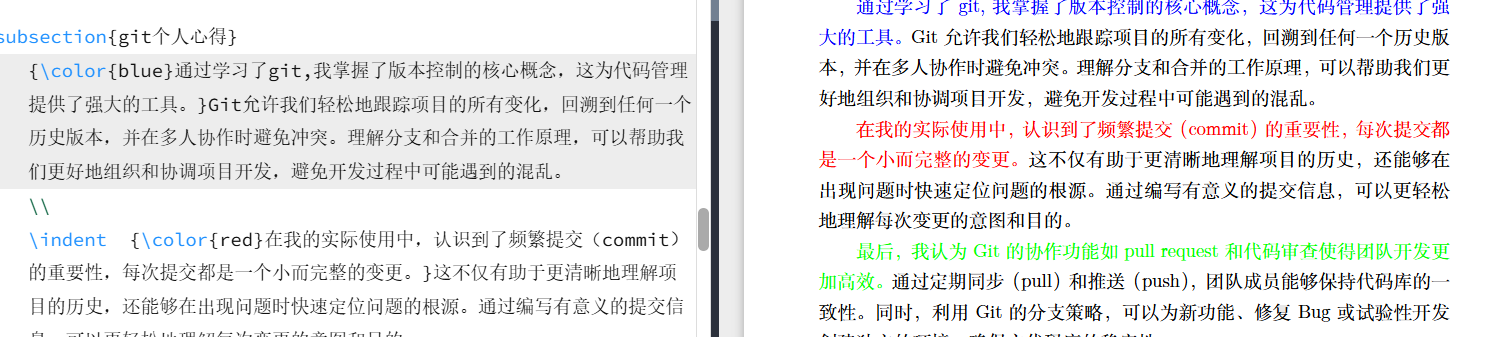
\includegraphics[width=1\textwidth]{屏幕截图 2024-08-29 201732.png}
  \caption{改变字体颜色}
    \end{figure}
\\
    \begin{figure}[H]
  \centering
  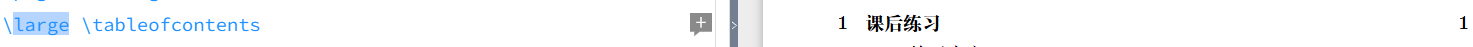
\includegraphics[width=1\textwidth]{屏幕截图 2024-08-29 201920.png}
  \caption{调整字体大小}
    \end{figure}

\subsection{latex个人心得}

{\color{red}学习LaTeX的过程中,我深刻体会到它作为一种强大排版工具的优势。LaTeX让你能够专注于内容本身,而不必为格式问题烦恼。它的高度可定制性和丰富的包支持,使得我可以创建专业水准的文档,无论是学术论文、演讲稿,还是复杂的数学公式,LaTeX都能轻松胜任。}

\\

{\color{blue}\indent 在实际使用中,掌握基本的命令和结构是关键。起初,LaTeX的语法可能显得有些繁琐,挺令人崩溃。但当熟悉了如何使用环境(environment)、命令和包(package),我会发现其强大的排版能力和一致性远超其他工具。特别是在处理长篇文档时,LaTeX的自动目录生成、引用管理和跨章节的引用功能尤为实用。}
    

\\
{\color{green}\indent  此外,良好的代码管理习惯同样重要。将文档拆分成多个部分,合理组织文件结构,可以提高项目的可维护性。通过使用版本控制工具如Git,你可以轻松跟踪文档的变化,确保每个版本的稳定性和可回溯性。整体来说,LaTeX不仅是一个文档排版工具,更是一种高效、专业的工作方式。}

\section{github仓库网址}
\href{https://github.com/newbeginnerlzh/git-task01.git}{\color{red}https://github.com/newbeginnerlzh/git-task01.git}
\end{document}